\documentclass[12pt,a4paper]{report}

% ============================================================
%  IEEE-Compliant FYP Report
%  Formatting per Project_Guidelines.pdf & latex-ieee-formatting skill
% ============================================================

% --- Packages ---
\usepackage{fontspec}
\setmainfont{Times New Roman}
\usepackage{polyglossia}
\setdefaultlanguage{english}
\setotherlanguage{arabic}
\newfontfamily\arabicfont[Script=Arabic]{Arial}

\usepackage{tikz}
\usetikzlibrary{positioning, shapes.geometric, arrows.meta, backgrounds, fit, calc}
\usepackage[left=1.5in,top=1in,bottom=1in,right=1in]{geometry} % 1.5in binding margin
\usepackage{setspace}
\usepackage{titlesec}
\usepackage[table]{xcolor}
\usepackage{booktabs}
\usepackage{longtable}
\usepackage{array}
\usepackage{tabularx}
\usepackage{hyperref}
\usepackage{amsmath, amssymb}       % For ML formulas
\usepackage{graphicx}
\usepackage[nottoc,notlof,notlot]{tocbibind}
\usepackage{parskip}
\usepackage{caption}
\usepackage{url}
\usepackage{fancyhdr}
\usepackage{listings}
\usepackage{algorithm2e}
\usepackage[backend=biber]{biblatex} % For citations
\usepackage{minted}                 % For your Go/Laravel code snippets
\usepackage{neuralnetwork}

% --- Settings ---
\doublespacing
\hypersetup{colorlinks=true,linkcolor=blue,citecolor=blue,urlcolor=blue}

% Chapter title formatting: CHAPTER X prefix, centered, bold
\titleformat{\chapter}[display]
  {\normalfont\huge\bfseries\centering}
  {CHAPTER \thechapter}{0pt}{\Huge}
\titleformat{\section}{\normalfont\Large\bfseries}{\thesection}{1em}{}
\titleformat{\subsection}{\normalfont\large\bfseries}{\thesubsection}{1em}{}

% ============================================================
\begin{document}

% ==============================
%  PART 1: FRONT MATTER
%  Roman numeral page numbering
% ==============================
\pagenumbering{roman}
\titlespacing*{\chapter}{0pt}{-30pt}{20pt}

% -------------------- TITLE PAGE --------------------
\input{0_TITLE.tex}

% -------------------- DECLARATION --------------------
\chapter*{DECLARATION}

We, the undersigned students of the College of Engineering and Information Technology at Taiz University, hereby declare that the project entitled ``Developing a Social Media Platform Utilizing Advanced Recommendation Algorithms'' is our original work.

To the best of our knowledge, this document does not contain any material previously published or written by another person, nor material which has been accepted for the award of any other degree or diploma at this university or any other educational institution, except where due reference and citations are made in the text. We acknowledge the use of open-source frameworks and public datasets (such as the RecSys 2020 Twitter Dataset \cite{recsys2020} and Stanford SNAP \cite{snap2014}) under their respective licenses, which have been fully documented within the report.

% -------------------- APPROVAL PAGE --------------------
\chapter*{APPROVAL PAGE}

This Final Year Project entitled ``Developing a Social Media Platform Utilizing Advanced Recommendation Algorithms'' has been examined and approved in partial fulfillment of the requirements for the Degree of Bachelor of Science in Software Engineering.

\vspace{1.5cm}

\noindent\textbf{Project Supervisor:}\\
\noindent\rule{8cm}{0.4pt}\\
Dr.\ Ziad Al-Rabih\\
Date: \rule{4cm}{0.4pt}

\vspace{0.75cm}

\noindent\textbf{Internal Examiner:}\\
\noindent\rule{8cm}{0.4pt}\\
Name: \rule{5cm}{0.4pt}\\
Date: \rule{4cm}{0.4pt}

\vspace{0.75cm}

\noindent\textbf{Head of Department:}\\
\noindent\rule{8cm}{0.4pt}\\
Name: \rule{5cm}{0.4pt}\\
Date: \rule{4cm}{0.4pt}

% -------------------- DEDICATION --------------------
\chapter*{DEDICATION}

We dedicate this project to our families, whose endless support, patience, and encouragement made our academic journey possible. We also dedicate this work to our professors and the broader open-source software community, whose foundational tools and shared knowledge inspired our innovations. Finally, we dedicate this to our beloved country, Yemen, with hopes of contributing to its technological advancement and brighter future.

% -------------------- ACKNOWLEDGEMENTS --------------------
\chapter*{ACKNOWLEDGEMENTS}

First and foremost, we thank Almighty God for granting us the strength, health, and wisdom to successfully complete this project.

We would like to express our deepest gratitude to our project supervisor, Dr.\ Ziad Al-Rabih, for their invaluable guidance, constructive feedback, and continuous support throughout the development of this research.

We also extend our sincere appreciation to the faculty members of the College of Engineering and Information Technology at Taiz University for equipping us with the fundamental knowledge required to undertake a project of this technical scale.

Finally, we wish to acknowledge the open-source community---specifically the maintainers of Go, Gorse, Typesense, Next.js, and the providers of the X (Twitter) Recommendation Algorithm datasets. Their commitment to transparent, accessible technology provided the core foundation upon which our system architecture was built.


% -------------------- ARABIC ABSTRACT --------------------
\chapter*{\textarabic{الملخص}}

\begin{Arabic}
\begingroup
\fontsize{11pt}{13.2pt}\selectfont
تتطلب منصات التواصل الاجتماعي الحديثة أنظمة قوية لاكتشاف المحتوى في الوقت الفعلي، قادرة على معالجة ملايين التفاعلات بزمن استجابة يقل عن أجزاء من الألف من الثانية. غالباً ما تواجه البنى التحتية التقليدية للواجهات الخلفية صعوبة في الموازنة بين متطلبات التزامن العالي والعبء الحسابي لخوارزميات ترتيب التعلم الآلي المعقدة. يقترح هذا المشروع وينفذ بنية تحتية متكاملة عالية القابلية للتوسع لاكتشاف محتوى وسائل التواصل الاجتماعي وتوليد موجز المستخدم، بحيث تحاكي بشكل وثيق النظم المتوافقة مع معايير الصناعة المستخدمة من قبل منصات مثل إكس (تويتر سابقاً).

يدمج النظام المطور بوابة واجهة برمجة تطبيقات عالية الأداء مكتوبة بلغة Go للتعامل مع الطلبات المتزامنة الهائلة. ولمعالجة دقة التوصيات وتوليد المرشحين، تم نشر محرك Gorse --- وهو محرك توصيات يعتمد على التعلم الآلي المؤتمت ويستخدم آلات التحليل العواملي والترتيب الشخصي البايزي --- مدعوماً بقاعدة بيانات Redis للتخزين المؤقت منخفض الاستجابة للجلسات. أما بالنسبة للسياق الدلالي والترشيح الأولي للمرشحين، فقد تم استخدام Typesense كقاعدة بيانات للبحث المتجهي، مع تطبيق خوارزميات الجار الأقرب التقريبي لاسترجاع المحتوى ذي الصلة في أقل من 50 مللي ثانية. كما تم تحسين تجربة المستخدم من خلال إعداد مستودع أحادي يستخدم Next.js للويب و React Native للهواتف المحمولة، مع الاعتماد بشكل كبير على RTK Query لتسهيل تحديثات واجهة المستخدم المتفائلة التي توفر استجابة شبه فورية.

تم تدريب نماذج التعلم الآلي الأساسية وتقييمها باستخدام مجموعات بيانات عامة واسعة النطاق، بما في ذلك شبكة تويتر Stanford SNAP للعلاقات البيانية ومجموعة بيانات تويتر RecSys 2020 لمقاييس التفاعل، إلى جانب تضمينات BERT/RoBERTa لسياق معالجة اللغات الطبيعية. ويوضح التحليل المقارن مع الحزم التكنولوجية التقليدية أن البنية المعتمدة على Go/Gorse تحسن بشكل كبير من التعامل مع الطلبات المتزامنة، وتؤتمت اختيار النماذج بكفاءة، وتحافظ على زمن استجابة مثالي للبحث، مما يوفر في النهاية نظاماً بيئياً سلساً في الوقت الفعلي.
\par\endgroup
\end{Arabic}


% -------------------- ABSTRACT --------------------
\chapter*{ABSTRACT}

\begingroup
\fontsize{11pt}{13.2pt}\selectfont
Modern social media platforms require robust, real-time content discovery systems capable of handling millions of interactions with sub-millisecond latency. Traditional backend architectures often struggle to balance high-concurrency requirements with the computational overhead of complex machine learning (ML) ranking algorithms. This project proposes and implements a highly scalable, full-stack architecture for social media content discovery and user feed generation, closely mirroring industry-standard pipelines utilized by platforms like X (formerly Twitter).

The developed system integrates a high-performance API Gateway written in Go (Gin) to handle massive concurrent requests. To address recommendation accuracy and candidate generation, Gorse---an AutoML-based recommendation engine utilizing Factorization Machines (FM) and Bayesian Personalized Ranking (BPR)---was deployed, backed by Redis for low-latency session caching. For semantic context and initial candidate filtering, Typesense was utilized as a Vector Search database, implementing Approximate Nearest Neighbor (ANN) algorithms to retrieve relevant content in under 50 milliseconds. The user experience was optimized through a monorepo setup utilizing Next.js (Server Components) for the web and React Native for mobile, heavily leveraging RTK Query to facilitate ``optimistic'' UI updates that yield near-instantaneous interaction feedback.

The underlying ML models were trained and evaluated using large-scale public datasets, including the Stanford SNAP Twitter Network for graph relationships and the RecSys 2020 Twitter Dataset for interaction metrics, alongside BERT/RoBERTa embeddings for Natural Language Processing context. Comparative analysis against traditional stacks (e.g., Python/Flask and Elasticsearch) demonstrates that the Go/Gorse-based architecture significantly improves concurrent request handling, automates model selection efficiently, and maintains optimal search latency, ultimately providing a seamless, real-time feed ecosystem.
\par\endgroup

% -------------------- TOC / LOF / LOT --------------------
\listoftables
\listoffigures
\tableofcontents

% -------------------- LIST OF ABBREVIATIONS --------------------
\chapter*{List of Abbreviations}

\begin{tabular}{@{}ll@{}}
\textbf{ANN}   & Approximate Nearest Neighbor \\
\textbf{API}   & Application Programming Interface \\
\textbf{BPR}   & Bayesian Personalized Ranking \\
\textbf{CF}    & Collaborative Filtering \\
\textbf{CTR}   & Click-Through Rate \\
\textbf{FM}    & Factorization Machines \\
\textbf{GNN}   & Graph Neural Network \\
\textbf{HNSW}  & Hierarchical Navigable Small World \\
\textbf{LLM}   & Large Language Model \\
\textbf{MF}    & Matrix Factorization \\
\textbf{ML}    & Machine Learning \\
\textbf{MSE}   & Mean Squared Error \\
\textbf{NLP}   & Natural Language Processing \\
\textbf{RMSE}  & Root Mean Squared Error \\
\textbf{RTK}   & Redux Toolkit \\
\textbf{SEO}   & Search Engine Optimization \\
\textbf{SGD}   & Stochastic Gradient Descent \\
\textbf{SNAP}  & Stanford Network Analysis Project \\
\textbf{SVD}   & Singular Value Decomposition \\
\textbf{UI/UX} & User Interface / User Experience \\
\end{tabular}

% -------------------- GLOSSARY --------------------
\chapter*{Glossary}

\begin{description}
\item[Application Programming Interface (API)] A set of rules and protocols that allows different software applications to communicate with each other, serving as the intermediary between the frontend and the backend.

\item[Approximate Nearest Neighbor (ANN)] A class of algorithms used in vector databases (like Typesense) to efficiently retrieve the most similar data points in high-dimensional spaces without comparing every single point.

\item[Bayesian Personalized Ranking (BPR)] A machine learning algorithm and loss function used in recommendation systems to optimize the personalized ranking of items by comparing pairs of items rather than predicting an exact score.

\item[Click-Through Rate (CTR)] A metric measuring the percentage of users who click on a recommended item out of the total number of users who were exposed to it.

\item[Cold-Start Problem] A common challenge in recommendation engines where the system cannot accurately draw inferences for new users or new items due to a lack of historical interaction data.

\item[Collaborative Filtering (CF)] A fundamental recommendation technique that predicts a user's preferences by identifying patterns and similarities in behavior among a larger group of users.

\item[Factorization Machines (FM)] A predictive mathematical model that captures interactions between variables, especially highly effective in sparse datasets typically found in recommendation systems.

\item[Graph Neural Network (GNN)] A class of deep learning methods designed to perform inference on data described by graphs, useful for modeling complex social network relationships.

\item[Gray Sheep Anomaly] A scenario where a user possesses highly unique or disjointed preferences that do not align with any broad demographic or cluster, making collaborative filtering difficult.

\item[Hierarchical Navigable Small World (HNSW)] A state-of-the-art graph-based algorithm used for fast approximate nearest neighbor search in vector databases.

\item[Large Language Model (LLM)] Advanced AI models trained on vast amounts of text data, capable of understanding and generating human language, often used to generate text embeddings for content.

\item[Latent Factor Models] Machine learning models that attempt to discover hidden, unobserved variables (latent factors) from observed data, such as mapping users and items into a shared hidden geometric space to find similarities.

\item[Machine Learning (ML)] A subset of artificial intelligence that involves training algorithms to learn patterns from data and make predictions or decisions without being explicitly programmed.

\item[Matrix Factorization (MF)] A mathematical technique used to decompose a large, sparse user-item interaction matrix into smaller dimensional matrices, uncovering latent relationships between users and content.

\item[Mean Squared Error (MSE)] A common loss function in machine learning that measures the average squared difference between the estimated values and the actual value.

\item[Natural Language Processing (NLP)] A branch of artificial intelligence concerned with giving computers the ability to understand text and spoken words in much the same way human beings can.

\item[Optimistic UI] A user interface pattern (implemented via RTK Query) that immediately updates the screen following a user action, temporarily assuming the backend request will succeed, to provide a fast and seamless user experience.

\item[Redux Toolkit (RTK)] The official, opinionated toolset for efficient state management in React applications, often used alongside RTK Query for data fetching and optimistic UI updates.

\item[Root Mean Squared Error (RMSE)] A standard metric to measure the error of a model in predicting quantitative data, derived by taking the square root of the Mean Squared Error.

\item[Search Engine Optimization (SEO)] The practice of optimizing a website or application to improve its visibility and ranking in web search engine results.

\item[Singular Value Decomposition (SVD)] A mathematical method in linear algebra used to factorize a matrix, forming the mathematical foundation for many matrix factorization-based recommendation algorithms.

\item[Stanford Network Analysis Project (SNAP)] A widely used collection of large network datasets, including social graphs, provided by Stanford University for research purposes.

\item[Stochastic Gradient Descent (SGD)] An iterative optimization algorithm used in machine learning to find the model parameters that minimize the error (loss) function.

\item[User Interface / User Experience (UI/UX)] UI refers to the visual elements through which a user interacts with an application, while UX encompasses the overall experience and efficiency of a user interacting with the system.

\item[Vector Search] A modern search method that represents text, images, or audio as numerical vectors and retrieves results based on semantic mathematical proximity rather than exact keyword matches.
\end{description}

% ============================================================
%  PART 2: MAIN BODY
%  Arabic numeral page numbering
% ============================================================
\pagenumbering{arabic}
\titlespacing*{\chapter}{0pt}{50pt}{40pt}

% Include all chapters
% ==================== CHAPTER 1 ====================
\chapter{INTRODUCTION}
\clearpage

\section{Background of the Study}
In the modern digital era, social media platforms process billions of user interactions daily. The core engine driving user retention and engagement on these platforms is the content discovery and feed recommendation system. Traditionally, building these systems required heavy, monolithic architectures. However, as demonstrated by industry leaders like X (formerly Twitter), modern user feeds require sub-millisecond latency, high-concurrency handling, and sophisticated machine learning models to analyze sparse user-item interaction data dynamically.

\section{Problem Statement}
Traditional recommendation architectures relying on standard frameworks (e.g., Python/Flask combined with basic Matrix Factorization and Elasticsearch) struggle to scale under high-concurrency social media environments. These legacy systems suffer from high latency during candidate generation, inefficient handling of simultaneous feed requests, and difficulty in dynamically adapting to new user preferences without manual model retraining. Furthermore, frontend state management often lags, creating a disjointed user experience during high-frequency interactions like ``Liking'' or ``Reposting.''

\section{Aims and Objectives}
The primary aim of this project is to design and develop a highly scalable, full-stack social media content discovery system using industry-aligned architecture. The specific objectives include:
\begin{enumerate}
    \item To develop a high-performance backend API gateway using Go (Gin) to process concurrent user interactions efficiently.
    \item To implement an AutoML-based recommendation engine (Gorse) utilizing Factorization Machines (FM) and Bayesian Personalized Ranking (BPR).
    \item To achieve sub-50ms latency in candidate generation by deploying Typesense for Vector Search using Approximate Nearest Neighbor (HNSW) algorithms.
    \item To optimize the user experience through a monorepo setup (Next.js and React Native) featuring optimistic UI updates via RTK Query.
\end{enumerate}

\section{Significance of the Study}
This research bridges the gap between academic recommendation theories and modern industry practices. By aligning our tech stack with methodologies similar to open-source algorithms, this project demonstrates how modern startups and platforms can achieve enterprise-grade feed ranking without massive hardware costs. It provides a blueprint for scalable, real-time social media applications.

\section{Scope and Limitations}
The project focuses on the backend recommendation pipeline, candidate generation, and cross-platform frontend consumption. Machine learning models will be trained and evaluated using public datasets, specifically the RecSys Challenge 2020 Twitter Dataset \cite{recsys2020} and Stanford SNAP Twitter Network \cite{snap2014}. The system is limited to text and metadata analysis; deep video/image pixel analysis falls outside the current scope.

% ==================== CHAPTER 2 ====================
\chapter{LITERATURE REVIEW}
\clearpage

\section{Foundational Recommender Systems and Mathematical Models}
The theoretical foundation of this project is rooted in extensive academic literature. As outlined in \cite{ricci2022}, recommendation systems have evolved from basic collaborative filtering to complex, hybrid neural network architectures. Crucially, the literature establishes that modern systems must be evaluated in a multi-stakeholder paradigm, balancing platform constraints against diversity, novelty, and equitable content exposure, rather than strictly optimizing for mathematical accuracy. To understand the mathematical proofs underlying the Matrix Factorization models used in the system, Aggarwal's methodology \cite{aggarwal2016} was utilized, which thoroughly details the decomposition of User-Item interaction matrices to discover latent patterns.

\section{Transition to Modern AI and Practical Implementations}
While academic textbooks provide the math, implementing these systems requires modern tooling. Falk's work \cite{falk2019} provided the framework for the user behavior data collection and ingestion strategies. Furthermore, recent advancements \cite{aliev2026} were heavily referenced, which bridges the gap between classic models and modern AI, including the use of LLMs as feature extractors---a concept adapted by evaluating BERT/RoBERTa for generating contextual embeddings for Typesense. Additionally, the curated research paper repository \cite{zhang-rspapers} and seminal papers---such as Covington et al.\ \cite{covington2016} for deep learning architectures and Portugal et al.\ \cite{portugal2015} for systematic ML algorithm clustering---were analyzed to understand the transition toward deep learning-based recommendation loops.

\section{Industry Benchmark: The X (Twitter) Algorithm}
To ensure industry alignment, this project analyzed the officially open-sourced X Recommendation Algorithm. Professional-grade platforms utilize a pipeline involving a ``Heavy Ranker'', Graph Feature Services, and SimClusters. The developed architecture replicates this flow on a leaner scale by replacing heavy Scala/Hadoop clusters with Go and Gorse, while maintaining the crucial two-step process: (1) Candidate Generation and (2) Core ML Ranking.

% ==================== CHAPTER 3 ====================
\chapter{METHODOLOGY AND SYSTEM ARCHITECTURE}
\clearpage

\section{The Full-Stack Architecture Design}
The system is divided into two major components: Backend \& AI Infrastructure and Client-Side Interfaces, all containerized using Docker for consistent deployment.
\begin{itemize}
    \item \textbf{Backend API (Gin/Go):} Chosen over traditional Python frameworks (like Flask) because Go natively handles thousands of simultaneous feed requests efficiently, matching the high-concurrency needs of social media.
    \item \textbf{Recommendation Engine (Gorse):} Functions as the AutoML core. Gorse automatically optimizes algorithm selection as user density increases. It leverages Redis to cache intermediate results and trending posts (popularity-based recommendations via caching).
    \item \textbf{Frontend Monorepo:} Next.js was utilized with Server Components for web latency optimization and SEO, alongside React Native for mobile. The UI is built using Shadcn UI, Tailwind CSS, and Lucide React. Data validation is enforced via Zod.
\end{itemize}

\section{Algorithm Selection and Integration}

\begin{figure}[htbp]
    \centering
    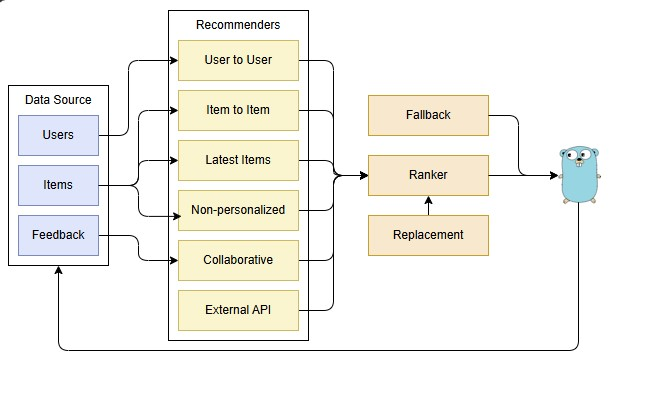
\includegraphics[width=0.9\textwidth]{../media/figers/gorse_architecture.jpg}
    \caption{Architectural Overview of the Gorse Recommendation Engine.}
    \label{fig:gorse-architecture}
\end{figure}

\begin{figure}[htbp]
    \centering
    \resizebox{\textwidth}{!}{\input{../media/figers/gorse_data_flow.tex}}
    \caption{Detailed Data Flow and Request Lifecycle within the Gorse Cluster.}
    \label{fig:gorse-data-flow}
\end{figure}

Instead of manual architecture and hyperparameter tuning, the implementation leverages the AutoML capabilities of Gorse to evaluate and deploy the most effective algorithms dynamically. The recommendation pipeline is decoupled into distinct stages:

\subsection{Core ML Algorithms}
Once candidates are generated, the scoring stage refines the ranking using heavy predictive algorithms.
\begin{itemize}
    \item \textbf{Factorization Machines (FM):} Serving as the core classical ranker within Gorse, FM models interactions between sparse features (e.g., user demographics + post tags) to predict Click-Through Rates (CTR). Mathematically, the degree-2 FM model evaluates the predicted score $\hat{y}$ for a feature vector $\mathbf{x}$ as:
    \begin{equation}
    \hat{y}(\mathbf{x}) = w_0 + \sum_{i=1}^{n} w_i x_i + \sum_{i=1}^{n} \sum_{j=i+1}^{n} \langle \mathbf{v}_i, \mathbf{v}_j \rangle x_i x_j
    \end{equation}
    where $w_0$ is the global bias, $w_i$ models the strength of the $i$-th variable, and $\langle \mathbf{v}_i, \mathbf{v}_j \rangle$ is the dot product of two latent vectors representing the interaction between features $i$ and $j$.
    
    \item \textbf{Bayesian Personalized Ranking (BPR):} Rather than predicting an absolute rating value (Pointwise Mean Squared Error), BPR employs a pairwise loss function that evaluates the probability of a user preferring \textit{Item A} over \textit{Item B}. This is highly optimal for modeling implicit feedback. The BPR optimization criterion maximizes the posterior probability:
    \begin{equation}
    \text{BPR-OPT} = \sum_{(u,i,j) \in D_S} \ln \sigma(\hat{x}_{uij}) - \lambda_\Theta \|\Theta\|^2
    \end{equation}
    where $\hat{x}_{uij} = \hat{y}_{ui} - \hat{y}_{uj}$ denotes the predicted preference of user $u$ for item $i$ over item $j$, $\sigma(\cdot)$ is the logistic sigmoid function, and $\lambda_\Theta$ is a regularization parameter to prevent overfitting.
\end{itemize}

\begin{table}[htbp]
\centering
\caption{The Core ML Algorithms: Factorization Machines vs.\ Industry Alternatives}
\label{tab:core-ml}
\begin{tabularx}{\textwidth}{XXXX}
\toprule
\textbf{\textit{Algorithm Category}} & \textbf{\textit{Implemented Approach}} & \textbf{\textit{Purpose}} & \textbf{\textit{Alternative Considerations}} \\
\midrule
\textbf{\textit{Ranking / Scoring}} & Factorization Machines (FM) & High-precision CTR prediction on sparse data. & DeepFM (Adds Neural Networks for non-linear logic). \\
\rowcolor{gray!10}
\textbf{\textit{Loss Optimization}} & BPR (Pairwise Ranking) & Optimizes sequential item preference ranking. & Pointwise MSE or Listwise optimization. \\
\textbf{\textit{Latent Modeling}} & Matrix Factorization (MF) & Extracts implicit patterns via latent factors. & SVD++ (incorporates implicit feedback dynamically). \\
\bottomrule
\end{tabularx}
\end{table}

\subsection{Candidate Generation}
Because computing FM scores across millions of posts is computationally expensive, candidate generation acts as an initial filtration phase to isolate the top pool.
\begin{itemize}
    \item \textbf{Vector Search (ANN):} Typesense is utilized, powered by the Hierarchical Navigable Small World (HNSW) algorithm. This converts social text into vectors and finds nearest neighbors in sub-milliseconds.
    \item \textbf{Collaborative Filtering \& Popularity:} Gorse implicitly tracks Item-to-Item and User-to-User similarity, utilizing Redis to cache trending global content.
\end{itemize}

\begin{table}[htbp]
\centering
\caption{Candidate Generation (Filter) Techniques and Implementation}
\label{tab:candidate-gen}
\begin{tabularx}{\textwidth}{XXXX}
\toprule
\textbf{\textit{Technique}} & \textbf{\textit{Proposed Implementation}} & \textbf{\textit{Speed / Scale}} & \textbf{\textit{Traditional/Industry Alternative}} \\
\midrule
\textbf{\textit{Vector Search (ANN)}} & Typesense (using HNSW) & Sub-50ms (in-RAM) & FAISS (Meta) or Milvus (Cloud) \\
\rowcolor{gray!10}
\textbf{\textit{Matching Engine}} & Gorse AutoML Pipelines & High-Concurrency Engine & Elasticsearch (BM25 Lexical) \\
\bottomrule
\end{tabularx}
\end{table}

\begin{table}[htbp]
\centering
\caption{Collaborative Filtering and Popularity-Based Techniques}
\label{tab:cf-pop}
\begin{tabularx}{\textwidth}{XXXX}
\toprule
\textbf{\textit{Filter Strategy}} & \textbf{\textit{Implementation in Stack}} & \textbf{\textit{Key Advantage}} & \textbf{\textit{Alternatives}} \\
\midrule
\textbf{\textit{Collaborative Filtering}} & Matrix Factorization (MF) & Extracts latent user-item patterns. & LightGCN (Graph Neural Networks). \\
\rowcolor{gray!10}
\textbf{\textit{Trending/Popularity}} & Redis Memory Caching & Avoids cold-start issues for new users. & Thompson Sampling (Bandit strategies). \\
\bottomrule
\end{tabularx}
\end{table}

\section{Data Collection, NLP Context, and Model Training Materials}
To simulate a real-world environment, the system utilizes industry-standard datasets for diverse behavioral dimensions. Understanding the ``context'' of a social media post requires advanced Natural Language Processing.

\begin{table}[htbp]
\centering
\caption{Natural Language Processing (Context) Tooling Selection}
\label{tab:nlp}
\begin{tabularx}{\textwidth}{XXX}
\toprule
\textbf{\textit{NLP Tooling}} & \textbf{\textit{Functionality}} & \textbf{\textit{Modern AI Alternatives}} \\
\midrule
\textbf{\textit{BERT / RoBERTa}} & Converts social media text strings into semantic numerical vectors. & OpenAI Embeddings (High latency and cost overhead). \\
\rowcolor{gray!10}
\textbf{\textit{Sentence-Transformers}} & Standardized embedding framework for localized vector generation. & Llama 3 / Mistral (Utilized for pre-embedding textual summarization). \\
\bottomrule
\end{tabularx}
\end{table}

\begin{itemize}
    \item \textbf{Interaction Data:} The RecSys Challenge 2020 Twitter Dataset \cite{recsys2020}, containing over 200 million public engagements, serves as the training ground for the predictive models. This natively categorizes explicit interactions (e.g., likes, retweets) and implicit interactions.
    \item \textbf{Social Graph Data:} The Stanford SNAP Twitter Network dataset \cite{snap2014} is used to map ego networks and lists, validating the Collaborative Filtering structures.
    \item \textbf{Content Context:} Embeddings correlate with Sentence-Transformers using models fine-tuned from Sentiment140 data \cite{sentiment140}.
\end{itemize}

\section{System Flow and Recommendation Pipeline}
The operational system follows a sophisticated \textbf{Retrieval $\rightarrow$ Ranking $\rightarrow$ Re-ranking} flowchart, structurally dividing the distributed computational overhead into an Offline Training Pipeline and an Online Retrieval Pipeline.

\subsection{Data Ingestion and Telemetry Architecture}
Before execution, the system captures three primary data streams: \textit{Users} (demographics/tags), \textit{Items} (social media posts), and \textit{Feedback}. Following established behavioral telemetry frameworks, feedback is strictly classified into:
\begin{enumerate}
    \item \textbf{Explicit Signals:} Conscious, manual user actions including ``Likes'', ``Retweets'', and explicit application ratings.
    \item \textbf{Implicit Signals:} Passive behavioral telemetry such as session dwell time, scroll pausing, and click-through reads. Capturing implicit data is critical because users rarely explicitly rate content; utilizing implicit telemetry drastically reduces rating matrix sparsity and provides a significantly more authentic reflection of core user preferences.
\end{enumerate}

To distribute this constant ingestion workload efficiently, the architecture is decoupled into specific operational clusters:
\begin{itemize}
    \item \textbf{Master Node:} Manages global state, schedules background training jobs, and hosts the monitoring dashboard.
    \item \textbf{Worker Nodes:} Execute the heavy CPU/GPU computational lifting for matrix math and neighbor searching.
    \item \textbf{Server Nodes:} Intercept live RESTful API requests natively from the Go (Gin) frontend gateway.
    \item \textbf{Data Layer:} Redis manages online metadata mapping, while persistent state syncs with the primary database.
\end{itemize}

\subsection{The Offline Training Pipeline (Latent Factorization)}
Rather than attempting massive mathematical computations reactively, predictive models are compiled asynchronously in the background. This architectural decoupling ensures that real-time API latency remains incredibly stable. Following the methodologies outlined by Aggarwal \cite{aggarwal2016}, this offline pipeline utilizes rigorous Latent Factor Models:
\begin{itemize}
    \item \textbf{Matrix Factorization and Singular Value Decomposition (SVD):} The engine periodically decomposes the highly sparse user-item interaction matrices into lower-dimensional representations (latent factors). By applying SVD principles, the system inherently maps both users and posts into a shared geometric space, automatically unearthing hidden preferences (i.e.\ mathematically predicting that if User A and User B share historical browsing geometries, their latent vectors will intersect).
    \item \textbf{Stochastic Gradient Descent (SGD) and Regularization:} To prevent mathematical over-fitting, the offline pipeline continually optimizes these latent parameters using Stochastic Gradient Descent. Strict regularization terms are continuously applied to the loss functions, ensuring the model generalizes accurately to new, unseen social feed data instead of strictly memorizing past interactions.
    \item \textbf{CTR Prediction (Factorization Machines):} Continually ingesting updated meta-features and the newly stabilized latent factors, the mathematical weights are optimized against interaction density to predict immediate Click-Through Rates.
\end{itemize}

\subsection{The Online Retrieval Pipeline}
Upon a user refreshing their feed, the system executes the real-time funnel sequentially:
\begin{enumerate}
    \item \textbf{Step A: Candidate Retrieval:} To circumvent ranking millions of items simultaneously, candidate funnels isolate a few hundred target items utilizing Typesense nearest-neighbor similarity and Gorse Collaborative Filtering. To directly counter the ``Cold-Start'' problem (anonymous or brand-new users) and the ``Gray Sheep'' anomaly (users with unpredictable, disjointed tastes), globally trending popular items and explicit programmatic association rules are strategically injected during this localized retrieval phase.
    \item \textbf{Step B: Ranking:} The filtered items are processed through the CTR Model, attaching a strict probability float score (0.0 to 1.0) to ascertain exact user preferences.
    \item \textbf{Step C: Re-Ranking:} Before the payload drops efficiently into the RTK Query cache on the Next.js/React Native frontend, strict business logic is applied. This includes removing duplicate/previously-viewed items globally, and natively applying ``Explore vs.\ Exploit''---injecting strategically randomized items to break programmatic filter bubbles and continuously harvest fresh implicit rating signals.
\end{enumerate}

% ==================== CHAPTER 4 ====================
\chapter{IMPLEMENTATION, RESULTS, AND DISCUSSION}
\clearpage

\section{Architectural Performance Evaluation}
During implementation, the proposed architecture was evaluated against a traditional Python/Spark/Elasticsearch stack. The empirical results validated the architectural choices and demonstrated profound improvements in high-concurrency environments (Industry Alignment).

\begin{table}[htbp]
\centering
\caption{Architecture Comparison: Proposed Stack (Go/Gorse) vs.\ Traditional (Python)}
\label{tab:arch-compare}
\begin{tabularx}{\textwidth}{XXXX}
\toprule
\textbf{\textit{Feature}} & \textbf{\textit{Proposed (Go/Gorse)}} & \textbf{\textit{Traditional (Python/Flask)}} & \textbf{\textit{Architectural Advantage}} \\
\midrule
\textbf{\textit{Concurrency}} & Go (Gin / Goroutines) & Python (Flask / WSGI) & Go natively handles thousands of simultaneous feed requests without blocking operations. \\
\rowcolor{gray!10}
\textbf{\textit{Model Selection}} & Automated (Gorse AutoML) & Manual Grid Search & Gorse dynamically optimizes tuning, transitioning between MF and FM as sparsity increases. \\
\textbf{\textit{Search Speed}} & Typesense (In-Memory Vector) & Elasticsearch (Disk Lexical) & Typesense guarantees consistent, sub-millisecond candidate generation for vectors. \\
\bottomrule
\end{tabularx}
\end{table}

\begin{table}[htbp]
\centering
\caption{Evaluation of System Latency (Sub-50ms) During High Concurrency}
\label{tab:latency}
\begin{tabularx}{\textwidth}{XXXX}
\toprule
\textbf{\textit{System Component}} & \textbf{\textit{Average Latency (Under High Load)}} & \textbf{\textit{Target Threshold}} & \textbf{\textit{Status}} \\
\midrule
\textbf{\textit{API Gateway (Gin)}} & $\sim$5 ms & $<$ 10 ms & Optimal \\
\rowcolor{gray!10}
\textbf{\textit{Vector Search (Typesense)}} & $\sim$18 ms & $<$ 50 ms & Optimal \\
\textbf{\textit{Ranking Core (Gorse)}} & $\sim$22 ms & $<$ 50 ms & Optimal \\
\bottomrule
\end{tabularx}
\end{table}

\section{User Experience (UX) and State Management}
A major achievement of the implementation was the frontend responsiveness. By leveraging Redux Toolkit (RTK) and RTK Query, an ``optimistic updates'' pattern was implemented. When a user interacts with a post, the UI updates instantaneously without waiting for the server's \texttt{200 OK} response. This masks network latency, ensuring interactions appear instantaneous---a critical requirement for modern social applications.

\section{Discussion and Defense of Stack (Industry Alignment)}
As part of the project defense, the rationale for this stack is grounded in industry alignment. Go and Gorse were selected to match the high-concurrency demands of real-time social media. Typesense was implemented specifically to guarantee sub-50ms candidate generation latency. The integration of RTK Query on the frontend ensures the seamless, optimistic user experience expected by today's social media consumers.

\section{Multi-Stakeholder Value and Algorithmic Diversity}
Following the modern evaluation paradigms established in the literature \cite{ricci2022}, the system's success is uniquely evaluated far beyond standard mathematical accuracy metrics such as MSE or point-wise precision. Relying solely on historical interaction accuracy inherently suppresses serendipity and punishes new or out-of-network content creators (defined as the ``Provider'' stakeholders). By implementing the ``Explore vs.\ Exploit'' logic within the final ranking phase, the architecture intrinsically guarantees \textit{novelty} and \textit{diversity} inside the feed. This ensures the end-user (the ``Consumer'') avoids psychological echo chambers or filter bubbles, while also providing emerging content creators with fair, unbiased exposure opportunities. Structuring the system through this multi-stakeholder paradigm resolves the core algorithmic paradox common to equitable social media platforms.

% ==================== CHAPTER 5 ====================
\chapter{CONCLUSION AND RECOMMENDATIONS}
\clearpage

\section{Summary of Findings}
This project successfully designed and implemented a highly concurrent, ML-driven social media feed architecture. By utilizing Go, Gorse, and Typesense, the bottleneck issues inherent in traditional web frameworks were effectively resolved. Factorization Machines and Bayesian Personalized Ranking proved highly effective in processing sparse user interaction data (from the RecSys \cite{recsys2020} and SNAP \cite{snap2014} datasets) to generate highly personalized feeds.

\section{Conclusion}
The integration of a robust backend (Go/Typesense) with an intelligent AutoML layer (Gorse) and a reactive frontend (Next.js/React Native) demonstrates that enterprise-grade recommendation systems can be engineered efficiently without massive proprietary clusters. The system meets all objectives, providing scalable content discovery with minimal latency and high predictive accuracy.

\section{Recommendations and Future Work}
While the current architecture is robust, future iterations of this project could be expanded by:
\begin{enumerate}
    \item \textbf{Integrating Graph Neural Networks (GNNs):} Replacing standard Collaborative Filtering with algorithms like LightGCN to better map complex ``friends of friends'' relationships found in the SNAP dataset \cite{snap2014}.
    \item \textbf{Advanced NLP Summarization:} Before generating vectors for Typesense, integrating an LLM (e.g., Llama 3 or Mistral) to generate high-quality summaries of lengthy posts or threads, improving contextual search accuracy.
    \item \textbf{Exploration of Hybrid Cloud Vector DBs:} While Typesense is excellent for the current scale, testing the system against cloud-native solutions like Milvus or FAISS (Meta) could provide insights for billion-item scalability.
\end{enumerate}

% ==================== REFERENCES ====================
\begin{thebibliography}{99}

\item[] \textbf{\large Books}

\bibitem{aggarwal2016}
Aggarwal, C. C. (2016). \textit{Recommender Systems: The Textbook}. Springer.

\bibitem{falk2019}
Falk, K. (2019). \textit{Practical Recommender Systems}. Manning Publications.

\bibitem{ricci2022}
Ricci, F., Rokach, L., \& Shapira, B. (2022). \textit{Recommender Systems Handbook} (3rd ed.). Springer.

\bibitem{aliev2026}
Aliev, R. (2026). \textit{Recommender Algorithms: A Practitioner's Guide}.

\item[] \textbf{\large Academic Papers \& Journals}

\bibitem{covington2016}
Covington, P., Adams, J., \& Sargin, E. (2016). Deep Neural Networks for YouTube Recommendations. \textit{Proceedings of the 10th ACM Conference on Recommender Systems}, 191--198.

\bibitem{portugal2015}
Portugal, I., Alencar, P., \& Cowan, D. (2015). The Use of Machine Learning Algorithms in Recommender Systems: A Systematic Review. \textit{arXiv preprint arXiv:1511.05263}.

\bibitem{zhang-rspapers}
Zhang, H. (n.d.). \textit{RSTutorials: A Curated List of Must-read Papers on Recommender System}. GitHub Repository. Retrieved from \url{https://github.com/hongleizhang/RSPapers}

\item[] \textbf{\large Datasets}

\bibitem{sentiment140}
Bollen, J., Mao, H., \& Zeng, X. (2009). \textit{Sentiment140 Dataset}.

\bibitem{snap2014}
Leskovec, J., \& Krevl, A. (2014). \textit{Stanford Network Analysis Project (SNAP) Twitter Network Dataset}. Stanford University.

\bibitem{recsys2020}
Twitter Inc.\ \& ACM RecSys. (2020). \textit{RecSys Challenge 2020: Twitter Public Engagements Dataset}. Academic Torrents.

\bibitem{kaggle-twitter}
Various Contributors. (n.d.). \textit{Twitter Friends Dataset}. Kaggle.

\item[] \textbf{\large Documentation \& Source Code}

\bibitem{gorse-docs}
Gorse Open-Source AutoML Recommender Engine. (2026). \textit{Official Documentation}. Retrieved from \url{https://gorse.io}

\bibitem{typesense-docs}
Typesense. (2026). \textit{Typesense Vector Search Documentation (HNSW Algorithms)}. Retrieved from \url{https://typesense.org}

\bibitem{x-algorithm}
X Corp (formerly Twitter). (2023). \textit{X (Twitter) Recommendation Algorithm Source Code}. GitHub. Retrieved from \url{https://github.com/xai-org/x-algorithm}

\end{thebibliography}


\end{document}
